\documentclass{standalone}
\usepackage[T1]{fontenc}
\usepackage[utf8]{inputenc}
\usepackage{pgf,tikz}
\usepackage{setspace}
\usepackage{pgfplots}
%\pgfplotsset{compat=1.9}

\usepgfplotslibrary{groupplots}

\begin{document}

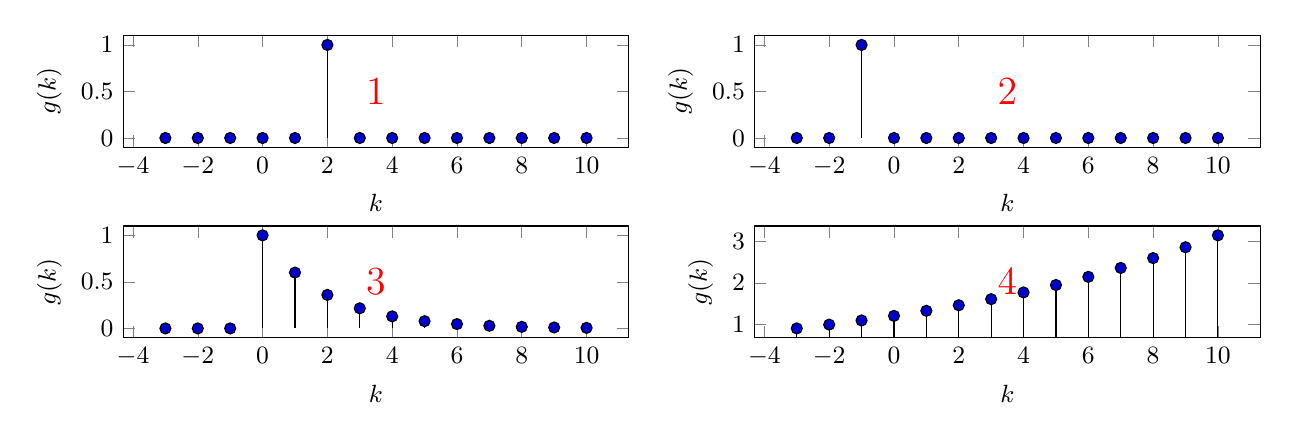
\begin{tikzpicture}
  \begin{groupplot}[
    group style={group size=2 by 2, horizontal sep=16mm,},
    height=3.0cm,width=8cm,
    /tikz/font=\small,
    %xtick={0,1,2,3, 4, 5},
    %xticklabels={0,$h$, $2h$, $3h$},
    % ytick=\empty,
    xlabel={$k$},
    ylabel={$g(k)$},
    %xmin=-0.6,
    %xmax=3.3
    % xmax=\axlim,
    % ymin=-\axlim,
    % ymax=\axlim,
    % axis lines=middle,
    ]

    \nextgroupplot
    \addplot+[black, ycomb, domain=-3:10, samples=14,variable=k] { (k==2)}; 
    \nextgroupplot
    \addplot+[black, ycomb, domain=-3:10, samples=14,variable=k] { (k==-1)}; 
    \nextgroupplot
    \addplot+[black, ycomb, domain=-3:10, samples=14,variable=k] { (k>=0)*pow(.6,k)}; 
    \nextgroupplot
    \addplot+[black, ycomb, domain=-3:10, samples=14,variable=k] { (k>=-3)*pow(1.1,k+2)}; 

    
  \end{groupplot}

   \node[red] at (group c1r1.center) {\Large \Romannum{1}};
  \node[red] at (group c2r1.center) {\Large \Romannum{2}};
  \node[red] at (group c1r2.center) {\Large \Romannum{3}};
  \node[red] at (group c2r2.center) {\Large \Romannum{4}};

\end{tikzpicture}
\end{document}
